\subsection {TopLevel}
\label{sec:TopLevel}
\sbol{TopLevel} is an abstract class that is extended by any \sbol{Identified} class that can be found at the top level of an SBOL document or file.
In other words, \sbol{TopLevel} objects are not nested inside any other object via \textit{composite aggregation} (represented by a filled diamond arrowhead on the UML diagrams).
Instead of nesting, composite \sbol{TopLevel} objects refer to subordinate \sbol{TopLevel} objects by their \sbol{URI}s using \textit{shared aggregation} (represented by an open-faced/non-filled diamond arrowhead on the UML diagrams).
The \sbol{TopLevel} classes defined in this specification are \sbol{Sequence}, \sbol{Component}, \sbol{Model}, \sbol{Collection}, \sbol{CombinatorialDerivation}, \sbol{Implementation}, \sbol{Attachment}, \sbol{ExperimentalData}, \prov{Activity}, \prov{Agent}, \prov{Plan} (see \ref{uml:toplevel}).
Each of these classes is described in more detail below, except for the classes from the provenance ontology (PROV-O), which are described in \ref{sec:provenance}.


\begin{figure}[ht]
\begin{center}
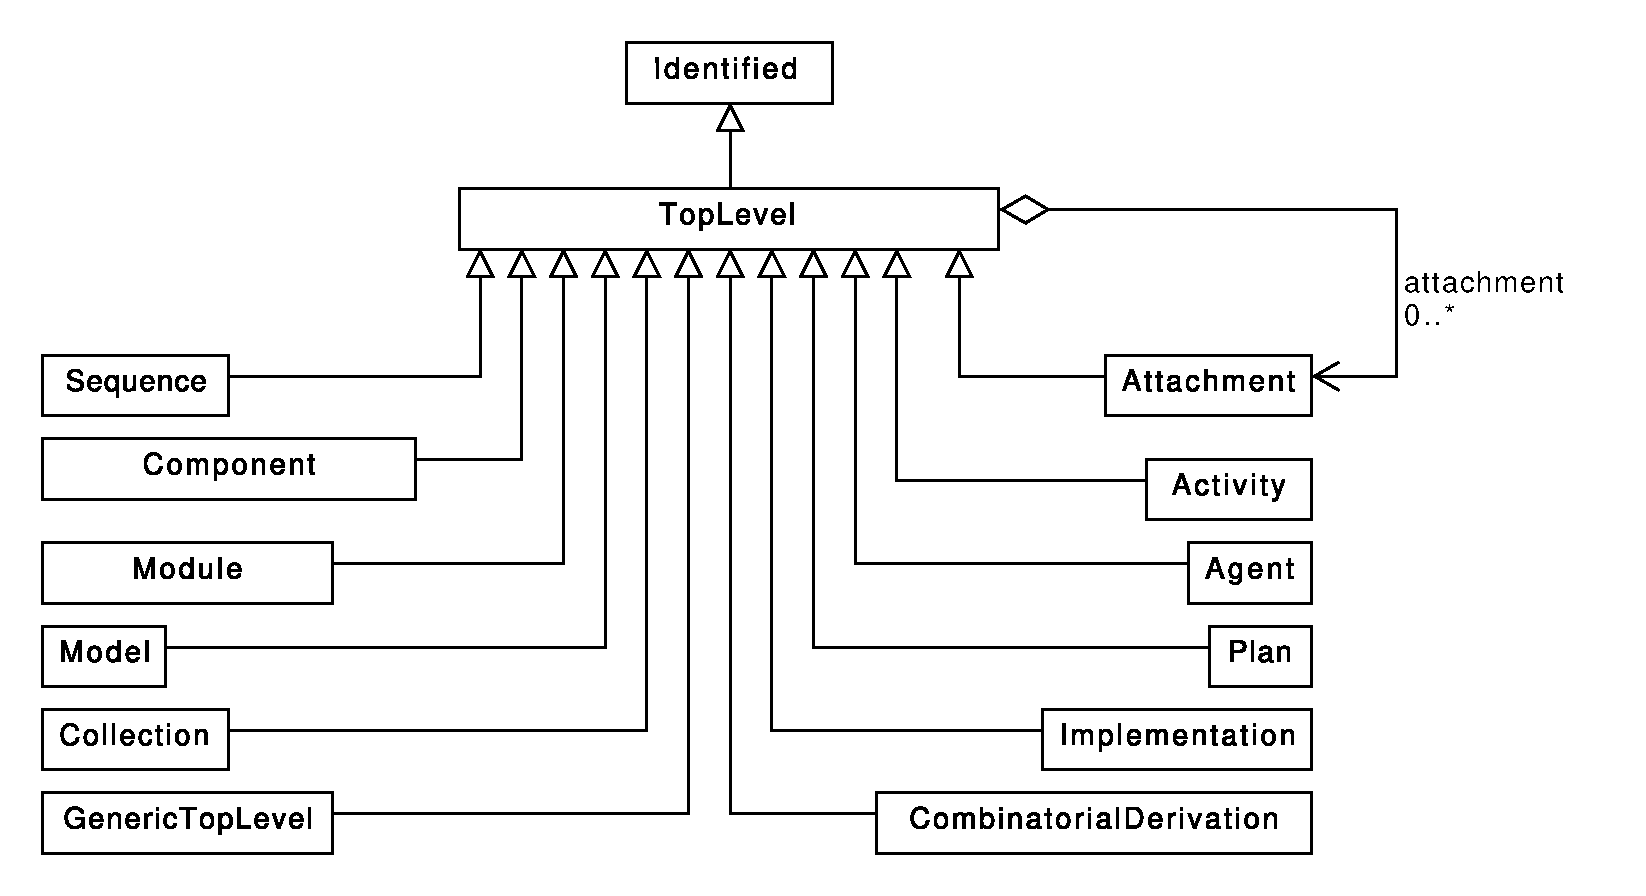
\includegraphics[width=\textwidth]{uml/toplevel}
\caption[]{Classes that inherit from the \sbol{TopLevel} abstract class.}
\label{uml:toplevel}
\end{center}
\end{figure}

\subparagraph{The hasNamespace property}
\label{sec:hasNamespace}
A \sbol{TopLevel} object MUST have precisely one \sbol{hasNamespace} property, pointing to the \sbol{Namespace} object that defines the namespace portion of URLs for this object and any child objects.
If the URI for the \sbol{TopLevel} object is a URL, then the URI of the \sbol{Namespace} MUST prefix match that URL.

Note that the requirement for a \sbol{hasNamespace} property holds even for objects with URIs that are not URLs, in order to allow them to be copied into datastores that use URLs.  In this case, however, there is no prefix requirement.


\subparagraph{The hasAttachment property}
\label{sec:hasAttachment}
A \sbol{TopLevel} object can have zero or more \sbol{hasAttachment} properties, each of type URI specifying an \sbol{Attachment} object. The \sbol{Attachment} class is described in more detail in~\ref{sec:Attachment}.


\subsection{Namespace}
\label{sec:Namespace}

The \sbol{Namespace} class is a simple placeholder that serves as a shared target for the \sbol{hasNamespace} properties of \sbol{TopLevel} objects.
Note that as a \sbol{TopLevel} object itself, a \sbol{Namespace} has a \sbol{hasNamespace} property that must point to itself.

